\chapter{排列和组合}
太极生两仪,两仪生四象,四象生八卦。其实易经里的乾、坎、艮、震、巽、离、坤、兑的可以认为是三个二进制组成的,八个卦象再\textbf{排列组合}又得到了六十四卦。
\begin{figure}[H]
\centering
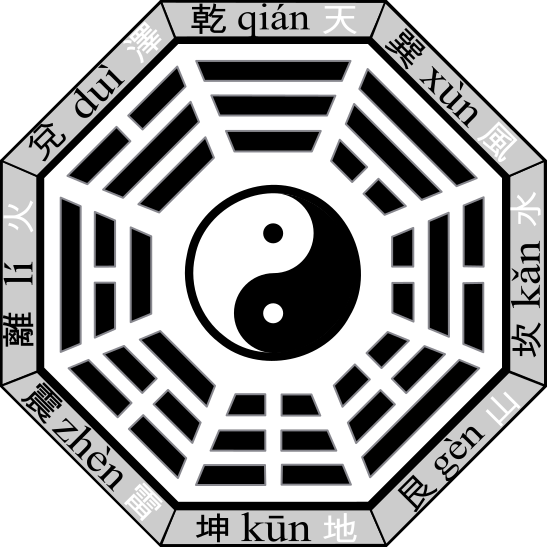
\includegraphics[width=0.3\textwidth]{bagua}
\end{figure}

\begin{todolist}
	\item 掌握\gls{factorial}的定义和运算规律
	\item 掌握\gls{permu}数的求算以及使用场景
	\item 掌握\gls{combi}数的求算以及使用场景
	\item 求算满足特定要求的排列方式
\end{todolist}
\clearpage

\section{先做一些微小的计算}
在正式利用排列组合求算之前,先要打好数学计算的基础

\subsection*{阶乘}
定义$n!$为:
\[
	n!=n\cdot (n-1)\cdot (n-2)\ldots\cdot 2 \cdot 1
\]

所以数字通过阶乘运算后会非常容易得到一个很大的数字,比如$10!=3628800$。阶乘可以用来表示将$n$个物体进行有序排序的方法的个数,比如将:$\mathcal{ABCDEFGH}$这$10$个字母排排列,可以产生多少种不同的搭配。这样的问题的答案就是$10!$。原因如下:将这一个任务分解成选择第一个字母,选择第二个字母,以此类推,总共有$10$个步骤。第一步有10个可选的字母,第二步有9个可选字母。因此利用\textbf{乘法法则}。所有的可行的数量为$10\times 9 \times 8 \ldots 1 = 10!$。而这个答案也可以认为是$10$个不同的字母形成的多少种顺序。

\begin{TaskBox}
在不适用计算器的情况下确定$30!$结果会有多少个$0$。
\end{TaskBox}

通过阶乘的定义,不难发现$n!=n\times (n-1)!$。如果这个特性可以继续推广的话,我们会得到一个比较重要的阶乘运算结果:
\[
	0!=\frac{1!}{1} = 1
\]
由此可见,$0!=1$。稍后我们将从排列的角度来解释为什么这个是reasonable的。


\section{排列数}
\gls{permu}是用于求算从$n$个物体当中有序排布其中的$r$个物体的总共可行的方法数。

如下图所示:
\begin{figure}[H]
\centering
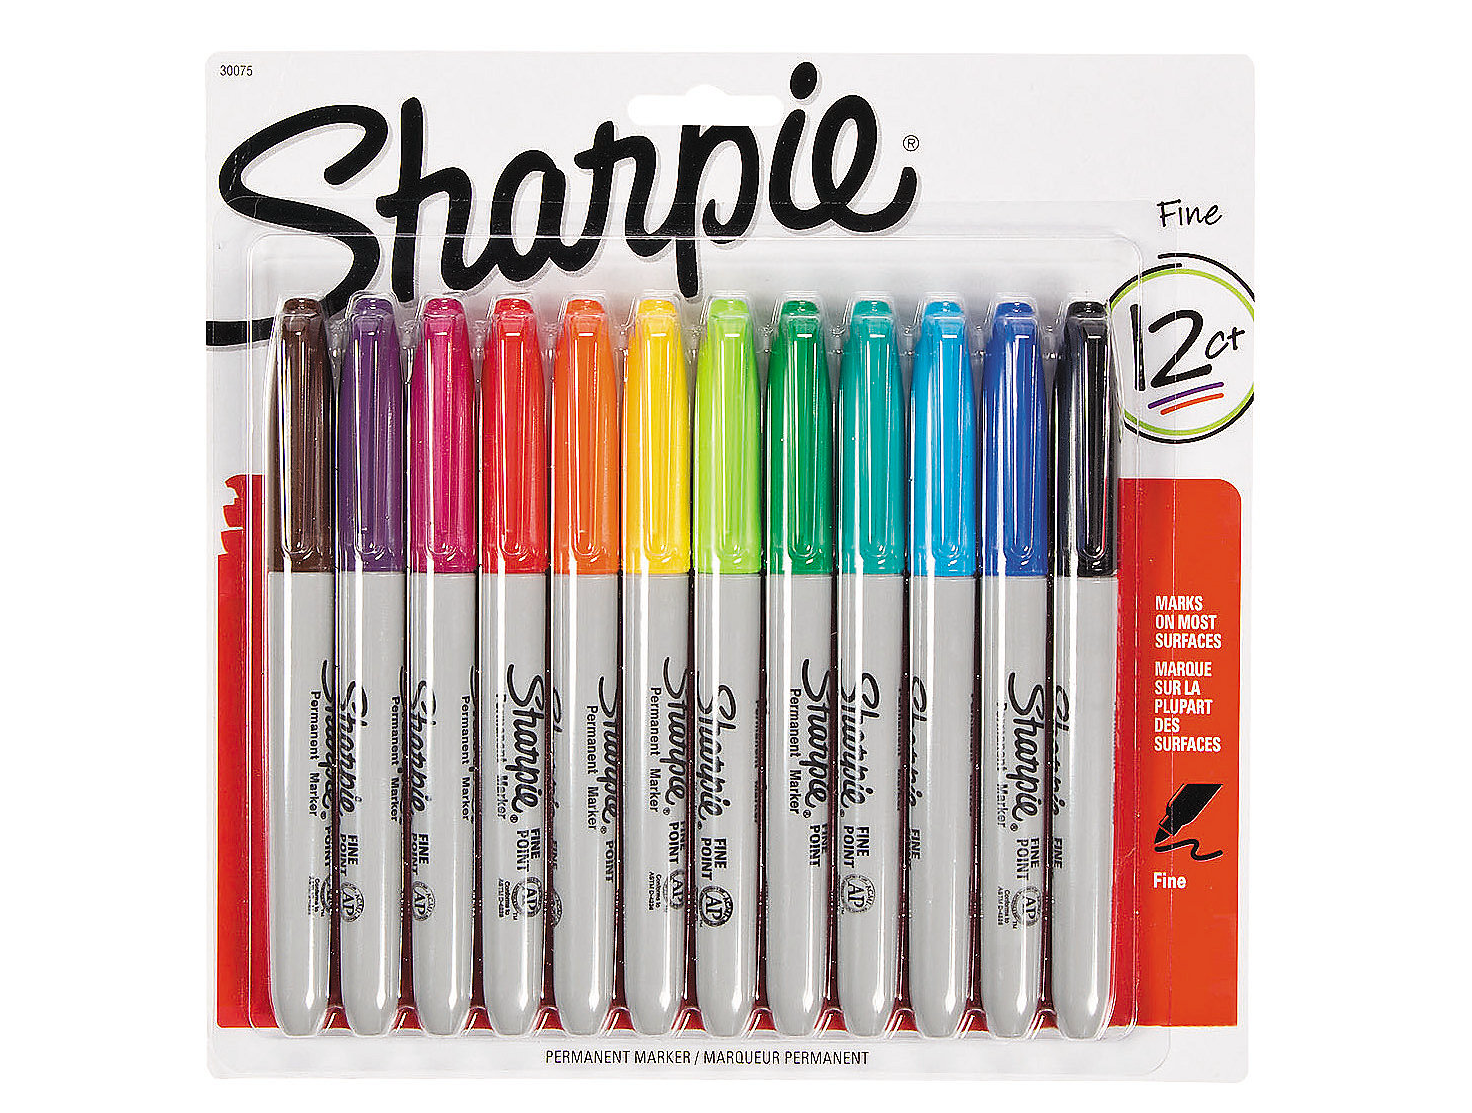
\includegraphics[width=0.8\textwidth]{marker}
\label{fig:marker}
\caption{12支不同颜色马克笔}
\end{figure}
如果将这$12$只不同颜色的马克笔不要求完全按照渐变色顺序,可以任意放置在包装袋中的话,就有$12!$种排列方式。因为第一支笔(最左侧的)可以有12种选择,第二支笔有11种选择,以此类推,并且根据\textbf{乘法法则},总共可能的个数为$12\times 11\times 10 \ldots \times 1 =12!$

但是,现在如果只需要排列其中的三支笔的话,肯定就没有这么多种排列方式了。不过思路还是一样的。最左侧的第一支笔依旧有12种选择,第二支10种,第三只还剩9种。所以总共的排列的方法数可以写作$12\times 11 \times 10$。为了方便简单,我们计作$^{12}P_3$ 数字$12$来自于总共有$12$个可选择对象,$3$来自与只需要排列其中的三只。完全可以把阶乘,排列数这些当成是一种运算符号,是为了省草稿纸的(手动狗头)。所以如果$^{n}P_{r}$\footnote{在部分教材中也会选择nPr这种写法}这样的形式来表示排列全部$12$支马克笔的话,其实就是$^{12}P_{12}$。

\subsubsection*{排列数用阶乘的表示方案}
$^{n}P_{r}$就是代表从$n$个对象当中,有序排列$r$个对象的方法个数。其计算会很浪费草稿纸,因为表达式如下:
\[
	^nP_r= \overbrace{n\times(n-1)\times (n-2).....\times(n+1-r)}^{r\text{ numbers}}
\]

如果$r$数据量小一点还好,但是一旦比较大的话就变得不``环保''了,而且数学家也不喜欢这种点点点点的不够具体形式,因此只需要简单的一乘一除就可以用阶乘进行表示$^nP_r$了。过程如下:
\begin{align*}
	^nP_r &= \overbrace{n\times(n-1)\times (n-2)\ldots\times(n+1-r)}^{r\text{ numbers}}\\
		  &= n\times(n-1)\times (n-2)\ldots \times(n+r-1) \times \frac{(n-r)\times (n-r-1) \ldots\times 1}{(n-r)\times (n-r-1) \ldots\times 1}\\
		  &= \frac{n\times(n-1)\times (n-2)\ldots \times(n+r-1)\times(n-r)\times (n-r-1) \ldots\times 1 }{(n-r)\times (n-r-1) \ldots\times 1}\\
		  &= \frac{n!}{(n-r)!}
\end{align*}

所以是不是变得非常的简单了。而且,这个公式也能够验证之前提到的$0!=1$的性质,因为$^nP_n=\frac{n!}{(n-n)!}=n!$所以$0!=1$。其实$0!=1$的含义也可以类推到对0个物体进行全排列,只有一种排列方式,就是什么不排。

\begin{TaskBox}
解释一下你所理解的乘法法则
\end{TaskBox}
\clearpage

\section{组合数}
参考上一节当中的\ref{fig:marker}图片,这次我们将不排列顺序,仅仅选择其中的三只笔,将会有多少种选择手段?很明显,第一支笔将会有12种选择,第二支笔将会有11种选择, 第三支是10种,第三只笔有9种,那这样不就和刚才的结果一样了吗?不,一个点很不相同,就是顺序。在之前Arrangement的情况当中,三支笔哪怕是完全同样的颜色,只要取出的顺序不一致,那么就会被认为是不同的排列方案。但是在现在的情况下,只要是同样的三种颜色就会被认为是一种方法。所以其最终结果数目肯定比$^{12}P_{3}$要少很多。至于少掉多少,来看下一部分

\subsection*{$r$个对象的重复}
%xcolor当中要调用dvi格式
在刚才的情境中,看看重复的次数。如果指定这三种颜色为\textcolor{Orange}{橙色},\textcolor{Yellow}{黄色},\textcolor{SeaGreen}{绿色}。那么三种颜色不同的顺序会有多少种\textbf{排列}?这个答案并不难:

罗列出所有结果:
\begin{enumerate}
	\item  \textcolor{Orange}{橙色},\textcolor{Yellow}{黄色},\textcolor{SeaGreen}{绿色}
	\item  \textcolor{Orange}{橙色},\textcolor{SeaGreen}{绿色},\textcolor{Yellow}{黄色}
	\item \textcolor{Yellow}{黄色},\textcolor{Orange}{橙色},\textcolor{SeaGreen}{绿色}
	\item \textcolor{Yellow}{黄色},\textcolor{SeaGreen}{绿色},\textcolor{Orange}{橙色}
	\item \textcolor{SeaGreen}{绿色},\textcolor{Orange}{橙色},\textcolor{Yellow}{黄色}
	\item \textcolor{SeaGreen}{绿色},\textcolor{Yellow}{黄色},\textcolor{Orange}{橙色}
\end{enumerate}
共计6种,而这个结果完全就是$3!$。也是可以从$^3P_3$推导而来的,相当于把三个物品进行排列,共计产生6种不同的顺序的方法。

因此当有$r$个对象需要重复的时候,产生的重复顺序就是
\[
	\framebox{^rP_r \quad\text{or } \quad r!}
\]

\subsection*{除法去重}
在解决组合类的问题当中,这一步是关键一步。$12$支笔选择$3$支的结果,完全可以等于$^{12}P_{3}$去除以三支笔先后顺序导致的重复。因此可以用$^{12}P_{3} \div 3!$。能够使用除法的原因,可以从乘法法则的逆向思考。排列12支笔当中的3支,可以分为两个步骤进行:\\
Step1 选出其中的需要排序的3支;\\
Step2 对选中的3支进行排列;

因此必定有step1所有的方法数 乘以 3!(step2的方法数)  等于 $^{12}P_{3}$
\begin{ExampleBox}
Find the number of ways in which all nine letters of the word TENNESSEE can be arranged without any other restrictions.
\makebox{}\hfill Adapted from 2015 winter qp 61 Q5
\tcblower
Step1 将TENNESSEE的所有字母,共9个做全排列,结果为$^9P_9$或者是$9!$ (默认前提,4个E字母和2个N字母,还有2个SS字母当成是不一样的。比如T\textcolor{red!75}{E}\textcolor{DarkOrange}{E}\textcolor{lime}{N}\textcolor{green}{N}\textcolor{RedOrange}{E}\textcolor{cyan}{S}\textcolor{SkyBlue}{S}\textcolor{YellowOrange}{E}\textcolor{yellow}{E})\\
Step2 去除由于E字母带来的重复,这个可想而知,之前强行将E看做是不一样的,我们进行了着色处理,但是想想一下,此刻突然变成了色盲,无论是T\textcolor{DarkOrange}{E}\textcolor{RedOrange}{E}\textcolor{green}{N}\textcolor{lime}{N}\textcolor{YellowOrange}{E}SS\textcolor{yellow}{E} 还是T\textcolor{RedOrange}{E}\textcolor{lime}{N}\textcolor{green}{N}\textcolor{DarkOrange}{E}SS\textcolor{yellow}{E}\textcolor{YellowOrange}{E}等等此时并没有任何区别了。四个E字母产生的顺序为$4!$\\

Step3 去除由于N字母带来的重复,同上一步,两个N字母产生的顺序为$2!$\\

Step4 去除由于S字母带来的重复,两个S字母产生的顺序为$2!$\\

因此最终结果为 $\frac{9!}{4!\times 2!\times 2!}=3780$
\end{ExampleBox}

可以用python跑的代码如下,纯粹暴力数。
\begin{verbatim}
from itertools import permutations
word = list(str(input("请输入字符")))
all_possible = list(permutations(word,len(word)))
result = []
count = 0
for permu in all_possible:
	if permu not in result:
		result.append(permu)
		#print(permu)
		count += 1
print(count)
\end{verbatim}

但是该代码的时间复杂度还有空间复杂度都比较大,并不是最快的方案,输出也不够美观,可以有很大的提升改进。

\subsection*{组合数和排列数的关系}
根据上面的推导,排列当中会有由于顺序带来的重复,利用除法去重之后,从12支笔当中选择3支的方案总数为$\frac{^{12}P_{3}}{3!}$。这样也可以认为是从12支笔一次性的拿取/选择/搭配组合3支笔的方案个数。因此计作$^{12}C_{3}$,称之为\gls{combi}。12和3只是一个例子,实际上这种计算方法可以沿用到任何数字当中。因此有:
\[
	^{n}C_{r}  = \frac{^{n}P_{r}}{r!} = \frac{n!}{(n-r)!\cdot r!}
\]

\subsection*{组合数的性质}
组合数有两个常用的性质会减小计算量。
第一个是$^{n}C_{r}=^{n}C_{n-r}$。其含义是从$n$个物体当中挑选$r$个物体的方法数目与挑选$n-r$个是一样的。所以还记得杨辉三角中,系数的是对称的吗?

第二个性质是$^{n}C_{0}=^{n}C_{n}=1$。其含义是从从$n$个物体当中挑选$0$个物体,或者$n$个物体的方法数目是1,即全不选、全都要
\begin{figure}[H]
\centering

\includegraphics[width=0.5\textwidth]{aobai}
\end{figure}

\begin{TaskBox}
利用$^{n}C_{r}$的计算公式证明上面的两个性质
\end{TaskBox}
\clearpage

\section{综合运用}
在目前的考试中,主要有以下的三类场景:
\begin{itemize}
	\item 字母的重新组合
	\item 数字搭配
	\item 人员排布和委员会
	\item 人员分配位置或者帐篷分配
\end{itemize}

涉及到的考察方法有:
\begin{itemize}
	\item 某些元素必须相邻;比如HAPPY字母重排中,要求两个字母P必须相邻;学生排队当中,两个女生闺蜜必须要相邻
	\item 某些元素必须间隔;比如UNTIL字母重排中,要求两个元音字母必须间隔;学生排队当中,两个情敌必须分割
	\item 委员会包含指定人物或者不能包含指定人物;比如委员会当中至少包含一个少数党派成员,或者保守党A不能与民主党B同时在委员会中
	\item 特定元素必须在指定位置;比如314529重排要求为偶数
	\item 与古典概率结合
\end{itemize}

针对以上的情景和考察方式,先看一些例题进行归纳

\subsection*{插空法解决相邻和不相邻问题}
相邻
\begin{ExampleBox}
The digits 1, 3, 5, 6, 6, 6, 8 can be arranged to form many different 7-digit numbers. How many of the 7-digit numbers have all the even digits together?
\tcblower
首先分析全部元素,奇数有3个,各不相同,偶数有4个,但是是3个6和1个8。题目要求所有偶数都是在一起的。可以按照如下的步骤进行执行。

Step1 将1 3 5这三个奇数进行排列。共计有$3!$种可行方法

Step2 将 6 6 6 8这四个偶数进行排列。共计有$\frac{4!}{3!}$,过程同之前的TENNESSEE。

Step3 将6668构成的整体插入到 1 3 5 这三个偶数形成了\textcolor{red}{四个}空隙中,选择四个空隙当中的任意一个都可以,因此有$^4C_1=4$种。

利用乘法原则将每个步骤可行的方案数相乘即为最后答案。$3!\times \frac{4!}{3!}\times ^4C_1=96$种
\end{ExampleBox}
时间非常空余的同学可以尝试写出这96种排列到底是什么

\begin{TaskBox}
如果题目限制条件改为all the even digits together and all the odd digits together. 答案应该是多少种?该如何分为步骤去讨论
\end{TaskBox}

\begin{ExampleBox}
In how many ways can the letters in the word SUCCESS be arranged if no two Ss are next to one another?
\tcblower
SUCCESS总共有7个字母,为实现任意三个S都是分开的。可以执行如下的步骤:

Step1 将 U C C E 四个字母进行排列,但是考虑到两个C字母的重复,共计有$\frac{4!}{2!}$种

Step2 将三个S插入到\textcolor{red}{五个}空隙中,并且由于三个字母都是S,因此没有先后顺序之分。所以可行的方法是$^5C_3$
两者直接相乘就可以
\end{ExampleBox}

\begin{TaskBox}
如果此题的限制条件为UE can not be next to each other。最终结果是多少?会在哪一步需要额外的限制条件
\end{TaskBox}

\subsection*{分类讨论的思想解决委员会问题}
\begin{ExampleBox}
A committee of $5$ people is to be chosen from $4$ men and $6$ women. William is one of the $4$ men and Mary is one of the $6$ women. Find the number of different committees that can be chosen if William and Mary refuse to be on the committee together.


\makebox{}\hfill Adapted from 2016 winter qp 63 Q1
\tcblower
此题的核心是William和Mary两人不能同时出现,因此,可以采用\textbf{分类讨论}的思想。分类为三种情况进行讨论:
\begin{itemize}
	\item Mary在committee当中
	\item William在committee当中
	\item 两个人都不在committee当中
\end{itemize}
所以,总共可行的方案数就是:
\[
	\overbrace{^1C_1}^{\text{选择Marry}}\cdot \overbrace{^{(10-2)}C_{(5-1)}}^{\text{从剩余8个人当中选择4个人}} + \overbrace{^1C_1}^{\text{选择William}}\cdot \overbrace{^{(10-2)}C_{(5-1)}}^{\text{从剩余8个人当中选择4个人}}+\overbrace{^{(10-2)}C_{5}}^{\text{从剩余8个人当中选择5个人}} = 196
\]
\end{ExampleBox}

\begin{TaskBox}
除了正面的分类讨论之外,此题也可以通过反向讨论,用总共可行的方案数减去两个人都在committe当中的方案数,尝试用这种方法完成此题。
\end{TaskBox}


\begin{ExampleBox}
A small aeroplane has $14$ seats for passengers. The seats are arranged in $4$ rows of $3$ seats and a back row of $2$ seats (see diagram). $12$ passengers board the aeroplane, consisting  of $2$ married couples (Mr and Mrs Lin and Mr and Mrs Brown), $5$ students and $3$ business people.
\begin{figure}[H]
\centering
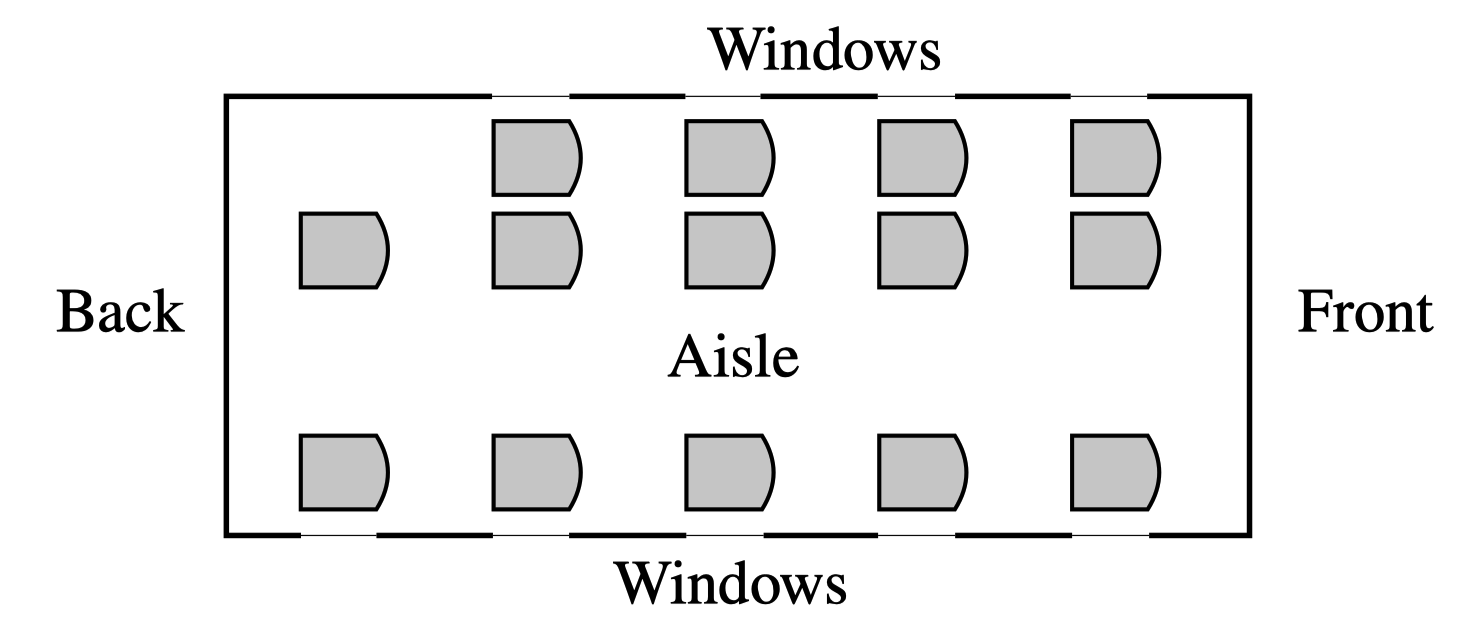
\includegraphics[width=0.3\textwidth]{planeseats}
\end{figure}
The $3$ business people sit in the front row. The $5$ students each sit at a window seat. Mr and Mrs Lin sit in the same row on the same side of the aisle. Mr and Mrs Brown sit in another row on the same side of the aisle. How many possible seating arrangements are there?
\makebox{}\hfill Adapted from 2010 winter qp 63 Q6
\tcblower
解决此题还是利用乘法法则:

Step1,三个商人的座次 $3!$\\
Step2, 五个学生的座次 $5!$\\
Step3, 当这八个人坐定之后,只剩下6个座位,刚好能形成3个靠过道的两连坐,供两对夫妇。因此安排为$^3P_2\times 2! \times 2!$ 后面两个$2!$表示夫妇两人一前一后的顺序,而$^3P_2$则是代表有先后顺序地排列两对夫妇至位置当中。\\

因此最后的结果为17280种
\end{ExampleBox}

\begin{SummBox}
这一类的问题对思维的逻辑性,分类讨论,反面讨论的要求很高,只能自己多多做题,见过各种类型之后才能豁然开朗,茅塞顿开。可以针对之前提到的几种类型的题目完成做题方法的总结。
\end{SummBox}
